\chapter{Implementation}
\section{Foreword}
This section serves as engineering documentation for the project. All data models in the codebase are thoroughly decorated with in-editor documentation using \texttt{JsDoc}. React's tree structure also naturally guides new contributors through the app's component hierarchy, and thus this chapter focuses on rationalising the design and infrastructure choices made throughout the project. A working familiarity with a few technologies is implicitly assumed:

\begin{itemize}
    \item Source and version control (Github)
    \item Front-end web development: HTML, CSS and Javascript
    \item Back-ends, databases and remote cloud services
\end{itemize}

For the sake of brevity, sections will contain links to documentation pages of relevant libraries. Since they are not academic references, documentation of relevant libraries will be referenced using footnotes or in-text links, which further facilitate easy, immediate reference.

The goal is to create a high-quality app platform that is built for legacy and continued work. The first step is therefore to implement previously non-existent development infrastructure, especially since the online nature of the new app involves secret keys which can be monetarily exploited if compromised. The previous version of the app is henceforth referred to as Sage, and the new app is referred to by its new name, Within.


\section{DevOps Implementations}
The following sections outline the focal points of the infrastructure and tooling choices made for Within from a DevOps engineer's perspective.


\subsection{Developer Workflow}
The code is currently hosted open-source on \href{https://github.com/Darrekt/within-react-native}{Github}. Source control systems often are the first line of defence in code deployment and Github offers features to allow developers to implement secure rules on their repositories. The rules for the Within project are listed below, and will be elaborated in further sections.

\begin{itemize}
    \item Secret keys are stored in non-readable repository secrets.
    \item Non-collaborators cannot push changes directly to the repository.
    \item Changes cannot be pushed to the \texttt{main} branch without all tests passing and an approving review from an approved author, who cannot be the one who submitted the pull request.
    \item The build on the \texttt{main} branch is automatically deployed as the latest release whenever a change is effected.
\end{itemize}

In order to correctly maximise the utility of these features, a developer workflow is outlined in the project \texttt{README}. Github unfortunately does not offer strict branch protection like other version control systems, and thus developers must adhere to these guidelines, as they are not strictly enforced by the system. Invited collaborators may clone the repository directly and develop features on a separate branch, which will be merged into a staging branch (\texttt{development-staging}) before being approved to \texttt{main}. Non-collaborators who wish to contribute may fork the repository and submit a pull request from their fork, as per open-source norms.


\subsection{Continuous Integration / Continuous Deployment Infrastructure}
Automated CI/CD tasks are run by commissioning remote machines to run scripted actions (often called ``jobs'') for a fee whenever the codebase is updated. For this reason, many CI/CD solutions are offered as add-ons or plugins to popular version control systems, so that they may be run as post-commit hooks. All jobs in this project are implemented with Github Actions. Each action is implemented in YAML syntax under the \texttt{.github/workflows} folder in the root of the project repository. Github actions provide unlimited compute minutes to open-source repositories and is very well-integrated into the Git ecosystem, making it the superior choice. Currently, the jobs take a total of about 20 minutes on each code change, which would easily exceed the quota for a private repository. If the project is to go closed-source in the future, it may be of interest to change to an alternate, paid solution such as Travis CI or CircleCI.


\subsection{Regression Testing and Runtime Stability}
A key tenet of the software development lifecycle is to test code before deploying it. To this end, this project uses the open-source Jest testing library by Facebook. Jest implements a configurable test suite which recursively searches an entire Javascript project directory for any files ending in the \texttt{.test.js} extension, and provides a declarative syntax for writing and running tests. Developers can write tests right alongside the code that it tests. Code regression is henceforth detected by running a single command, and Jest displays a full breakdown of any test that failed as a result of recent code changes. The test suite is automatically run with every commit on the \texttt{main} and \texttt{development-staging} branches of the repository, and will cause the jobs running them to produce an error whenever the test suite fails.

Javascript as a language is dynamically typed and thus highly prone to runtime errors. This motivates the use of Typescript and immutable data. We will later see examples of how using strongly type-checked immutable data structures to track the state of the app greatly reduces the occurence of runtime errors that would have otherwise have been very difficult to detect.


\subsection{Build Stability}
\begin{figure}[h]
    \begin{center}
        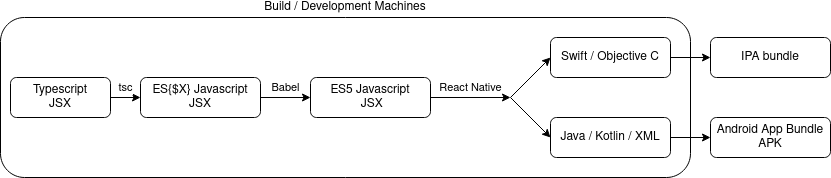
\includegraphics[scale=0.55]{images/app_build_path.png}
    \end{center}
    \caption{An example of the application build process.}
    \label{fig:app_build_process}
\end{figure}

React Native transpiles a React-syntaxed JavaScript codebase into an Android Kotlin project or an iOS project in Objective C. Figure \ref{fig:app_build_process} shows the build process of the toolchain involved in this application. Each step in the build process in this case involves a source-to-source compiler, which has to bridge semantic equivalents and substitutes between languages and frameworks. Having a long toolchain of different open-source components results in an unreliable build process which can fail if any dependencies along the toolchain fail for any reason.

True to form, throughout the development of this project, there were many instances in which the project would suddenly fail to build without any change in the codebase. Most frustratingly, the project involves writing platform-specific code, which adds another dimension along which a developer could cause the project build to fail. The long toolchain involved in the project build results in enormously long stack traces, which result in a situations where a developer cannot possibly know if the project is now failing to build as a result of their own changes, or a dependency breaking along the chain. Almost every time, the cause of build failure was a version dependency change in one very small library along the toolchain.

A naive solution would be to require the developer to run a script which builds app bundles for both platforms before pushing code to source control. However, building app bundles often takes a few minutes for each platform, which is extremely disruptive when developing small, rapid changes.

To address this issue, two automated jobs are defined in \texttt{android.yml} and \texttt{ios.yml}. The two jobs build the installation binaries for both native operating systems on cloud-connected build machines and throw an error if any of them fail, storing full trace logs in the job history on Github. Building the app requires the firebase configuration file, which contains secret keys and are not included in the source code. The firebase configuration files are first compressed into a tar archive, passphrase-encrypted with GPG and then uploaded to the repository root as \texttt{services.tar.gpg}. The passphrase is then kept as a repository secret, and loaded into an environment variable to decrypt and extract the configuration files on the build machine.

Developers can sign up for email-updates via the Github repository, which allows them to be immediately notified of a build failure. They can then immediately work on understanding if the failure was due to the most recent change, or an unexpected change in the React Native dependency chain.


\subsection{Product Deployment}
Presently, the app is not deployed on any public stores due to the release process requiring a significant investment which is outside the scope of the project. Releasing the app on either store requires a monetary investment for a developer account (USD\$125), a privacy policy hosted on an owned domain and a collection of assets for a store page listing. As a proof-of-concept and temporary workaround, the job implemented in \texttt{releasedraft.yml} automatically builds a release binary of the app whenever a change is successfully pushed to the \texttt{main} branch.

Building a release APK requires an app to be signed using a consistent set of keys as proof-of-work from the developer. These keys are contained in a keystore, which is encoded as a base64 string and then stored as a repository secret. The decryption passphrase is similarly stored as a repository secret, and both are loaded into environment variables for decryption on the build machine. Once the app is built and signed, the resulting build artefact (the release APK) is released on the repository with a new tag. In the future, this should be updated to use the API of the respective app stores to automate the release process.


\section{Developer Documentation}
Instead of exhaustively documenting screen flow which is best left to a live demo, the documentation in the sections to follow will detail the implemented features of the app in an order which is conducive to onboarding a new developer. New developers should adhere strictly to the contributing guidelines in the Github repository README. The documentation contained herein is by no means exhaustive, and will not fill in the gaps of knowledge for a new developer attempting to understand the repository. All linked documentation therefore serves as a starting point for further reading, and unfamiliar terms should be researched and understood before proceeding, if encountered at any point.

\subsection{Background Information}
\subsubsection{A brief tour of React}
React.JS is a library which introduces a declarative syntax for making responsive user interfaces on the web. Readers familiar with web technologies will be familiar with the Document Object Model (DOM), which simply describes the layout of a webpage in a tree-like structure. React allows a developer to declare `what' should appear on screen, which is `rendered' as a virtual DOM. This virtual DOM is then compared with what is presently on the user's screen (the actual DOM) using a process called reconciliation, in which only the differing elements between the two trees are identified and re-rendered. This results in minimal computation to achieve the desired change in the user interface without requiring a page refresh on behalf of the user, and the result is a single-page application (SPA), which continues to be the dominant design for parts of many modern websites.

The paradigm of `thinking in React' has now become so popular that React is a dominant presence in modern web stacks, and a highly in-demand skill for developers. Reactive paradigms have been further extended to new libraries such as React Native, which has an almost identical developer experience to React.JS, but transpiles down into native code for multiple platforms. React Native reads and largely feels like working in React.JS, but introduces a set of components which act as wrappers around native APIs to produce a codebase which has one consistent syntax which renders an app across multiple devices, and enables business logic to be entirely contained in JavaScript. There are naturally exceptions to this, such as when some APIs are only avaiable on one native OS and not the other, as we will see later.

As mentioned before, Within also makes extensive use of TypeScript (TS), which greatly increases code clarity and reduces runtime errors using compile-time type-checks, at the cost of writing slightly more upfront code. Since TypeScript is a typed superset of JavaScript (JS), this means that all valid JS code is valid TS code, and the result is a natural learning curve which a given develop can lean into as much as they prefer.

The root React node is contained in \texttt{App.tsx}, which contains other setup code for libraries which require initialisation outside of the standard React component lifecycle. Before proceeding, developers should read the documentation links below, as these concepts are heavily used in this repository. At minimum, a thourough understanding of the React component life cycle, as well as the \texttt{useEffect} post-render hook are required to understand the sections to come.

\begin{itemize}
    \item \href{https://reactjs.org/docs/hello-world.html}{React Docs} - the starting point for any React developer. Read all main concepts.
    \item \href{https://blog.isquaredsoftware.com/2020/05/blogged-answers-a-mostly-complete-guide-to-react-rendering-behavior/#rendering-process-overview}{A guide to React's rendering behaviour}
    \item \href{https://reactjs.org/docs/context.html}{React Context documentation}. Context is heavily used to pass data downwards through the component tree without having to bloat an entire chain of component props.
    \item \href{https://reactjs.org/docs/hooks-intro.html}{React Hooks documentation}. Hooks in React are a concise way of using component lifecycle methods and other React utilities without having to create a verbose class-based component.
    \item \href{https://www.typescriptlang.org/docs/}{Typescript Docs}
\end{itemize}

\subsubsection{App Navigation}
Navigation loosely refers to the practice of directing the user to different parts of the app using a visual experience. All navigation is implemented with the React-navigation\footnote{\href{https://reactnavigation.org}{React Navigation documentation}} library, which implements conditionally rendered fullscreen pages based on named routes. All routes are contained and enumerated in \texttt{navConstants.ts}.

\subsubsection{Global App State}
Within is a write-heavy application, with state that changes on every interaction. Such state needs to be accessible in different parts of the component tree, motivating the use of a single, global state provided by context at the root of the tree. However, global states require careful management and needs to be mutated in a stable manner to prevent crashing the app. All of these problems are solved by the Redux paradigm, which promotes the use of a single, immutable state contained in a plain, serializable JavaScript object.

\begin{figure}[h]
    \begin{center}
        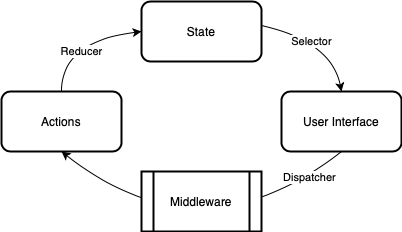
\includegraphics[scale=0.55]{images/redux_state.png}
    \end{center}
    \caption{The state-component lifecycle with Redux}
    \label{fig:redux_state}
\end{figure}

Redux\footnote{\href{https://redux.js.org/usage/usage-with-typescript}{Redux documentation}} is a state-management paradigm which generates new states based only on the current state and a descriptive action, the processing of which is handled by a pure function that contains no side-effects (called a reducer). App state is purely contained within a serializable JavaScript plain object, which means the state will not contain any moving or self-mutating parts. The resulting state is always predictable and thus easy to debug. Since states simply transform from one to another in a sequence instead of mutating, state-recording debugging methods such as time-travel debugging, crash logging and an undo history are easily implementable.

Since its inception, Redux has developed a rich ecosystem, which has unfortunately resulted in unstandardised documentation and practices. The current best practice for using Redux is to use Redux-toolkit\footnote{\href{https://redux-toolkit.js.org}{Redux toolkit documentation}} along with library-specific bindings, and thus Within implements global state using Redux-toolkit and React-redux\footnote{\href{https://react-redux.js.org}{React-redux documentation}}.

Figure \ref{fig:redux_state} shows the data flow for Within using Redux. Relevant parts of the state are read from the store into React components using selectors. Interactive parts of the user interface dispatch actions, which may or may not be intercepted by middleware to execute side-effects before passing the action on to the reducers, which generate a new state based on the old state and the dispatched action.

The React-redux library allows us to provide a global store through context at the root level of the app. The reference of the store object itself does not change when actions are dispatched, and components down the tree use selectors to select specific parts of the global state to ``listen'' to. This results in a performant user interface which only re-renders the relevant parts of the component tree when relevant bits of the app state change, instead of the entire tree. Similarly, the dispatch function which is used to dispatch actions for the store is also provided globally at the root using context. It is noteworthy at this point that both \texttt{useAppDispatch} and \texttt{useAppSelector} are pre-typed wrappers\footnote{\href{https://redux.js.org/usage/usage-with-typescript}{Redux usage with Typescript}} around their base counterparts from the Redux library.

The global state in this case is also split into segmented parts using reducer-splitting, in which each part of the app state is handled by a sub-reducer. All redux and state-related implementations are contained in the \texttt{redux} folder, and the \texttt{rootReducer} combines the subreducers using ES6 object property-value shorthand. All selectors can be found in the \texttt{selectors.ts} file.


\subsection{Authentication and Identity Management}
Data synchronisation is achieved through a user's unique ID, which is unified across all their logins. The secure login is implemented through the Firebase SDK using the React-native-firebase bindings\footnote{\href{https://rnfirebase.io}{React-native-firebase documentation}}, which provides a single point of unified identity management using either email credentials or one of the supported providers. Users are able to access their data and have the same experience across devices after logging in.

While Firebase offers support for third-party login providers, these are unfortunately unavailable in the scope of this project due to the lack of presence on an app store. Apple devices require any app offering provider sign-ins to offer AppleID sign-ins first, which require a verified developer account and a published app on the App Store for security reasons. However, a traditional email and password style sign-in is fully implemented.

In Within, the user's login status is held in the \texttt{appSettings}-related reducers. A single listener in the \texttt{StackScreens.tsx} component dispatches an action whenever the user's Firebase login state changes.


\subsection{Structuring Productivity in Data}
\subsubsection{Motivation}
As discussed previously, a key factor in successful self-regulation is the amount of cognitive effort required to successfully execute a task. Therefore, procrastination is best avoided if users are able to consistently plan their work schedules into small, manageable tasks which can be completed in a single 25-minute focus interval. In Sage, this was entirely the user's responsibility as only to-dos could be created without any form of structure other than daily recurring tasks. Within seeks to introduce a more deliberate structure that emulates real project work, with a more longitudinal time scope and time-sensitive deliverables in-between.

\subsubsection{Initial Data Model}
\begin{figure}[h]
    \begin{center}
        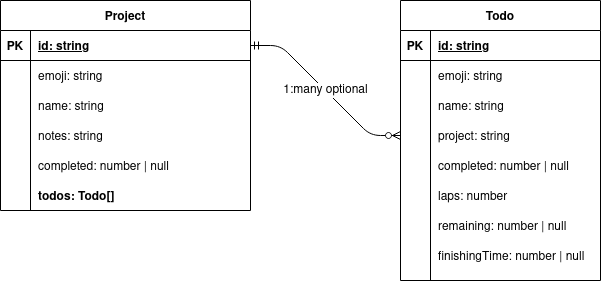
\includegraphics[scale=0.5]{images/initial_data_model.png}
    \end{center}
    \caption{The initial data model.}
    \label{fig:initial_data_model}
\end{figure}

Figure \ref{fig:initial_data_model} shows the Entity-relationship (ER) model to support projects and to-dos. This schema is easy to implement using foreign-key relations in an SQL-like database. However, noSQL stores such as Firestore often use composition to capture relationships. This is reflected in the fact that a Project contains an array of Todos, which are serialised to raw string values for storage in the database. In an SQL environment, this would be captured purely using a foreign-key relation between Projects and Todos. This replication (signified in \textbf{bold}) has been left intact, since it does not change any of the factors affecting pricing by any significant amount, and is useful in helping developers understand the relation between the two entities, should the system migrate to an SQL datastore later on.

\subsubsection{Revised Data Model}
\begin{figure}[h]
    \begin{center}
        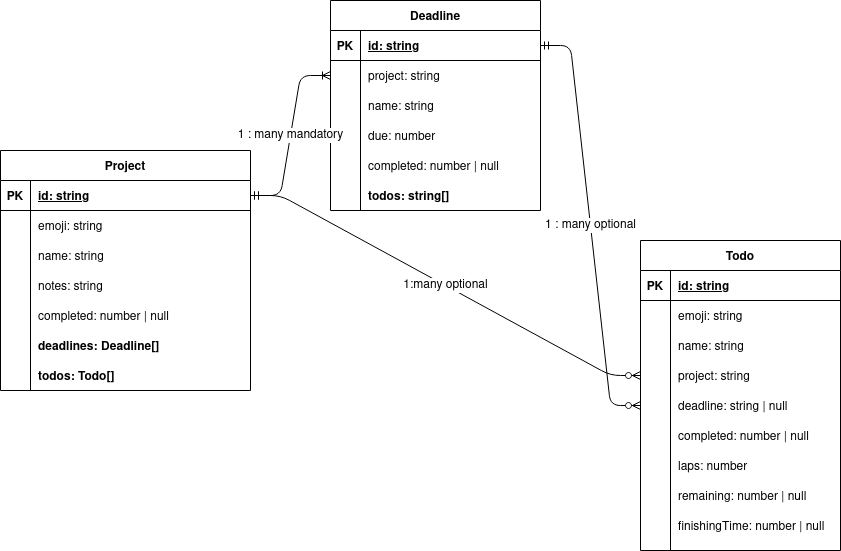
\includegraphics[scale=0.5]{images/final_data_model.png}
    \end{center}
    \caption{The current data model.}
    \label{fig:app_current_data_model}
\end{figure}

Projects needed to be broken down further into multiple deadlines, and a given deadline in focus had to be further decomposed into individual tasks on a per-session basis. Figure \ref{fig:app_current_data_model} shows the ER model for the updated schema. This model allows for a structured breakdown of complex tasks, modelled after a typical student or academic's workload.

\subsubsection{Syncing through snapshot listeners}
Firebase bills developers off of three key metrics: reads, writes and network eggress\footnote{\href{https://cloud.google.com/firestore/quotas}{Firebase quotas documentation}}. JSON-like objects are stored as documents in named collections, and documents may themselves hold subcollections. Therefore, an obvious was to optimise the schema for minimal reads is to hold more information within a single document. Reads and writes are optimised by serialising small objects into \texttt{string} representations, which can then be kept in arrays under larger entities. In Firebase, all deadlines and todos are held under a single project's document. The user's work data is therefore encapsulated in an array of \texttt{Projects}. Changes to any entity (Todo, Deadline or Project) also consequently only cost 1 document write under this schema.

Firebase offers snapshot listener functions as part of its Javascript API. These follow a publish / subscribe (pub/sub) model where a subscription function is passed a callback to execute. Real-time synchronisation is achieved by attaching a function to a listener in \texttt{StackScreens.tsx} which dispatches an action to load the updated app state into whenever the database is updated, in a process called ``hydration''. The app state stored in the database is taken to be the single source of truth, and actions therefore cause changes in the app by writing directly to the database, triggering a hydration. This, however, is an asynchronous action which happens over a network. Since Redux reducers are meant to be pure functions without side-effects, there is a need to ``intercept'' the action and perform the database write as an asynchronous side-effect before dispatching the action on to the store. The Redux-thunk middleware\footnote{\href{https://github.com/reduxjs/redux-thunk}{Redux thunk documentation}} is built for this purpose. All database-sensitive actions are therefore implemented as thunks in files called \texttt{thunks.ts}, which are categorised by their respective slice reducers under the \texttt{redux} folder.


\subsection{Do-not-disturb mode}
Preventing notifications from disturbing a user is one of the key functions of the app. The native Android SDK gives a developer the ability to invoke a callback function whenever a notification is fired by the system. The previous notification-blocking functionality thus worked by adding code within this callback to dismiss the notification as soon as it was fired. This implementation has 2 fatal flaws: firstly, the asynchronous nature of the callback invocation meant that there would be non-deterministic edge cases in which running tasks on the main thread would delay the dismissal of the notification, therefore firing too late to dismiss it and allowing the notification through. Secondly, the dismissal of a notification meant that a user would not see them after the work interval is complete, potentially causing the user to miss important messages or calls.

A more suitable implementation that fixes both of these faults lies in the Do-not-disturb (DnD) functionality provided by the Android OS. DnD mode suppresses notifications while active, preventing attention-grabbing features such as sound, vibration and the notification LED on the phone face. This has obvious applications for users who are driving, in important meetings, or otherwise wishing to be undisturbed. All notifications received in this mode are still visible to a user who deliberately picks up the phone and checks the notification inbox after the fact, which means users still have access to any important pieces of information delivered during the interval.

The challenge now is accessing native android APIs from within React Native. As Figure \ref{fig:app_build_process} showed previously, the entire app is written in Typescript. However, React Native offers a \texttt{NativeModules} feature which allows developers to write native code modules which may be accessed across the language gap. Full documentation is available in the \href{https://reactnative.dev/docs/native-modules-intro}{React Native guide}. From here, turning on Do-not-disturb mode programmatically is a matter of navigating the Android APIs. The full code is available in \texttt{DnDMode.java}.


\subsection{Disruption Detection}
Even with notifications disabled, users are likely to be distracted when faced with roadblocks or difficult tasks, and may flee the app to seek momentary relief on social media or other distracting apps. A solution to this would be if the Within app could detect when such distractions occur, and prompt the user's pre-frontal cortex to wrest back control.

Apps on phones typically adopt one of three states: they are either foregrounded, backgrounded or inactive. React Native provides nice utilities around these states \footnote{React Native AppState documentation available \href{https://reactnative.dev/docs/next/appstate}{here}}, allowing the developer to attach callback functions when such state transitions are triggered.

The relevant listener is subscribed in \texttt{TodoTimer.tsx}. The relevant code attaches an event handler in a post-render hook using \texttt{useEffect}. Since the timer component re-renders whenever the selected task changes, it is necessary to re-subscribe the listener whenever the timer re-renders, and the selected todo is therefore included in the dependency array.

The listener uses the \texttt{react-native-push-notification} library to push a notification to the user whenever the app takes on a non-active state while the timer is running. For this to be fully effective, however, users must manually allow the Within app to push notifications through do-not-disturb mode, which would be active when the timer is running. There is no way for the developer to enable this programmatically, and thus the user has to be clearly guided through this process as part of a future onboarding flow.

\section{User Interface Design}
Instead of aiming to develop a fancy user interface full of bells and whistles, Within aims to re-implement a simple UI with minimal clutter and good foundations in interactivity and visualisation. In this section, we will explore how Within incorporates concepts from interactivity experts such as Donald Norman and Niklas Elmqvist into its UI. Since this is not a study in human-computer interaction, we will simply make an attempt to implement the UI in a way which conforms with the guidelines explored below without studying them in-depth.

A fluid interface, as defined by Elmqvist \cite{elmqvist2011fluid}, is an interface which promotes flow \cite{csikszentmihalyi1990flow}, supports direct manipulation\cite{shneiderman19931} and minimises both of Norman's \cite{norman1986user} gulfs of action.

\paragraph{Gulfs of Action} Donald Norman defines two `gulfs' of action: the gulf of evaluation, which refers to the difference between the system state and the user's perception of it, and the gulf of execution, which refers to the difference between what the user perceives they are able to do and what the system permits. A large gap in either of these gulfs results in confusion or frustration for the user, as more cognitive resources are required for them to reconcile the differences between the information presented to them and what is actually happening in the system.

\paragraph{Flow} The concept of flow has been highly applied in many user-interaction systems, and has become a key principle of addictive design. Yet, flow itself is a very abstract concept which has no formal definition, but refers generally to the act of a user staying highly engaged and focused on a given activity. Csikszentmihalyi \cite{csikszentmihalyi1990flow} states a few factors for flow which Elmqvist \cite{elmqvist2011fluid} highlights as particularly relevant for the creation of fluid interfaces:

\begin{itemize}
    \item Balanced challenge - The skill required to actuate an intention and the user's skill should be matched. In modern app design, as we have reviewed previously, often the goal is to completely eliminate any challenge required to actuate an intention.
    \item Concentration - Structuring the app experience in a way that permits a high degree of focus on a limited field of attention.
    \item Transformation of time - Users should be able to immerse in the app experience and disregard external stimuli, essentially losing track of time.
    \item Prompt feedback and sense of control - Instant feedback of the effect of a user's action minimises the gulfs of action, giving the user a sense of control and resulting in what many users will simply feed back as an ``intuitive feel''.
\end{itemize}

These concepts are difficult to measure quantitatively and are circularly dependent, but can be intuitively felt in many of today's modern products: consider a slot machine, social media app or modern video game. The challenge in this case would be to reproduce such an experience in an app which takes on a much more boring and less stimulating context (doing work instead of engaging with friends or simulated challenges).

\begin{figure}[h]
    \centering
    \begin{subfigure}{0.4\linewidth}
        \centering
        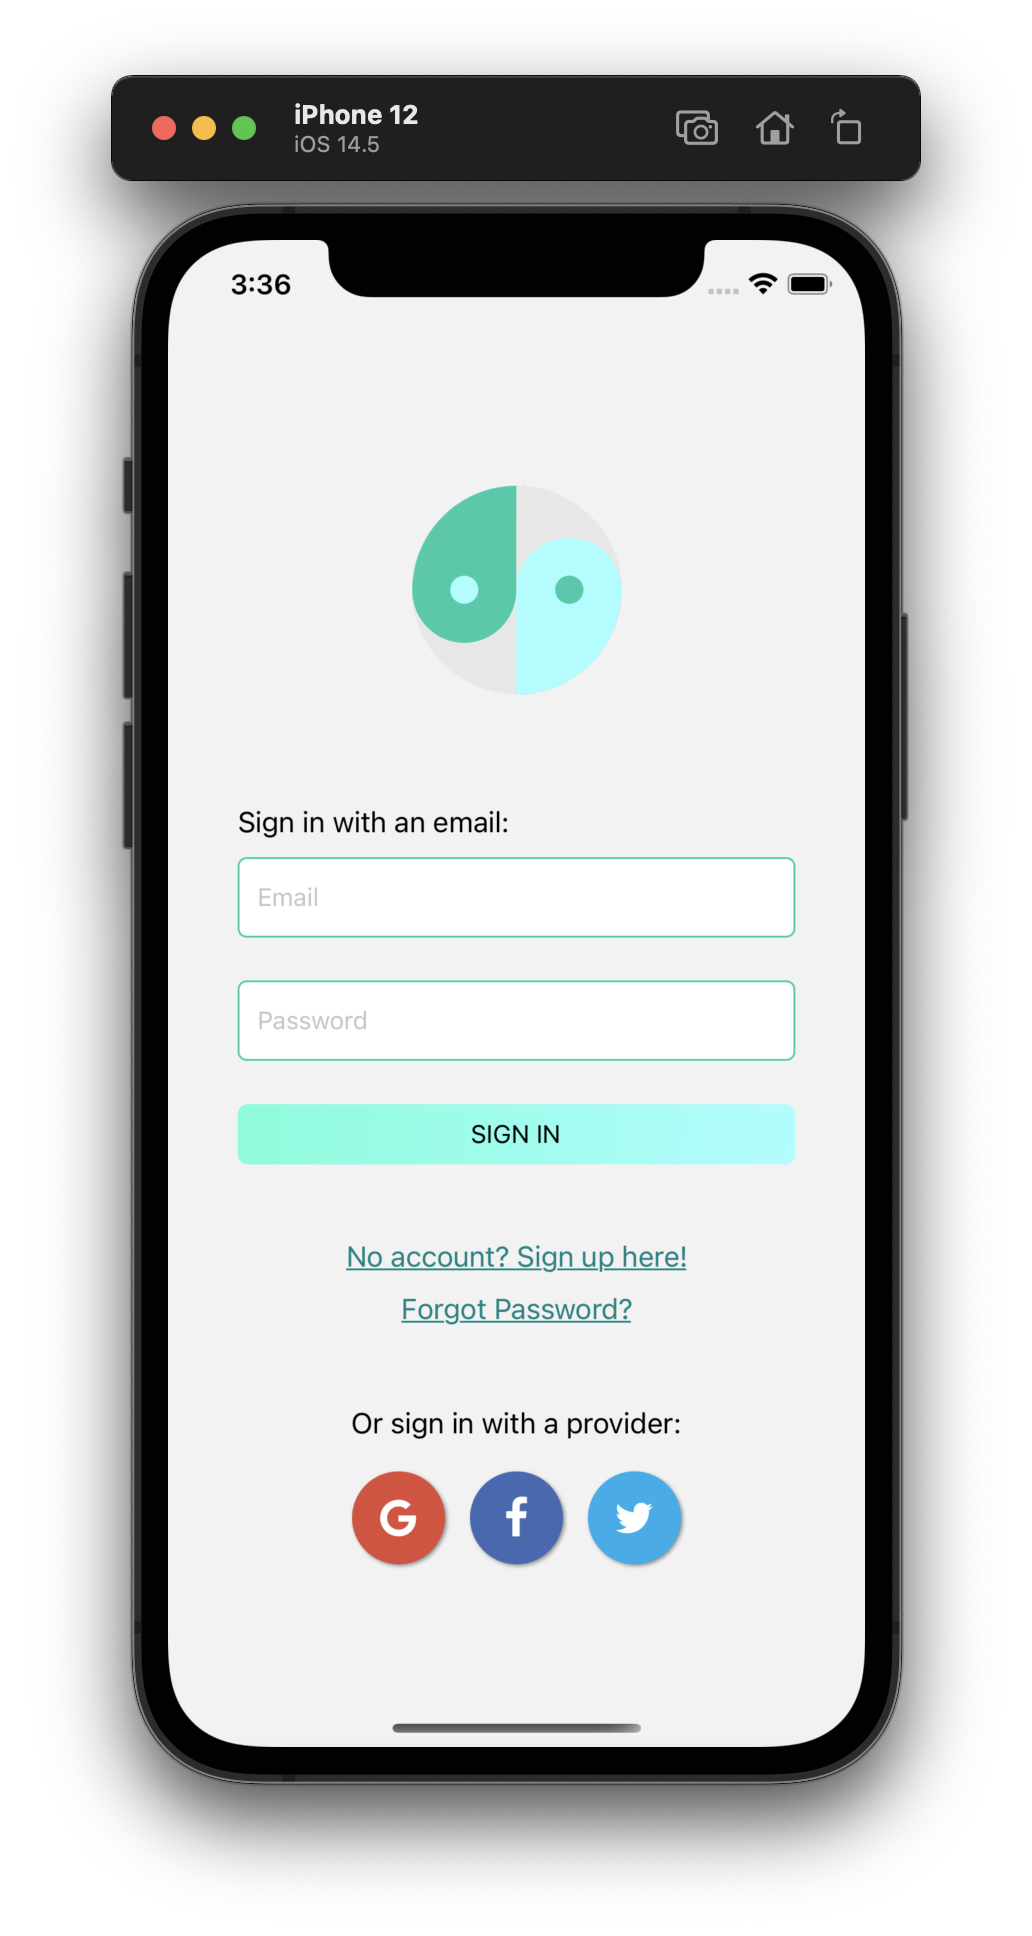
\includegraphics[scale=0.25]{images/login_screen.png}
        \caption{The Within login screen}
        \label{fig:login_screen}
    \end{subfigure}%
    \begin{subfigure}{0.4\linewidth}
        \centering
        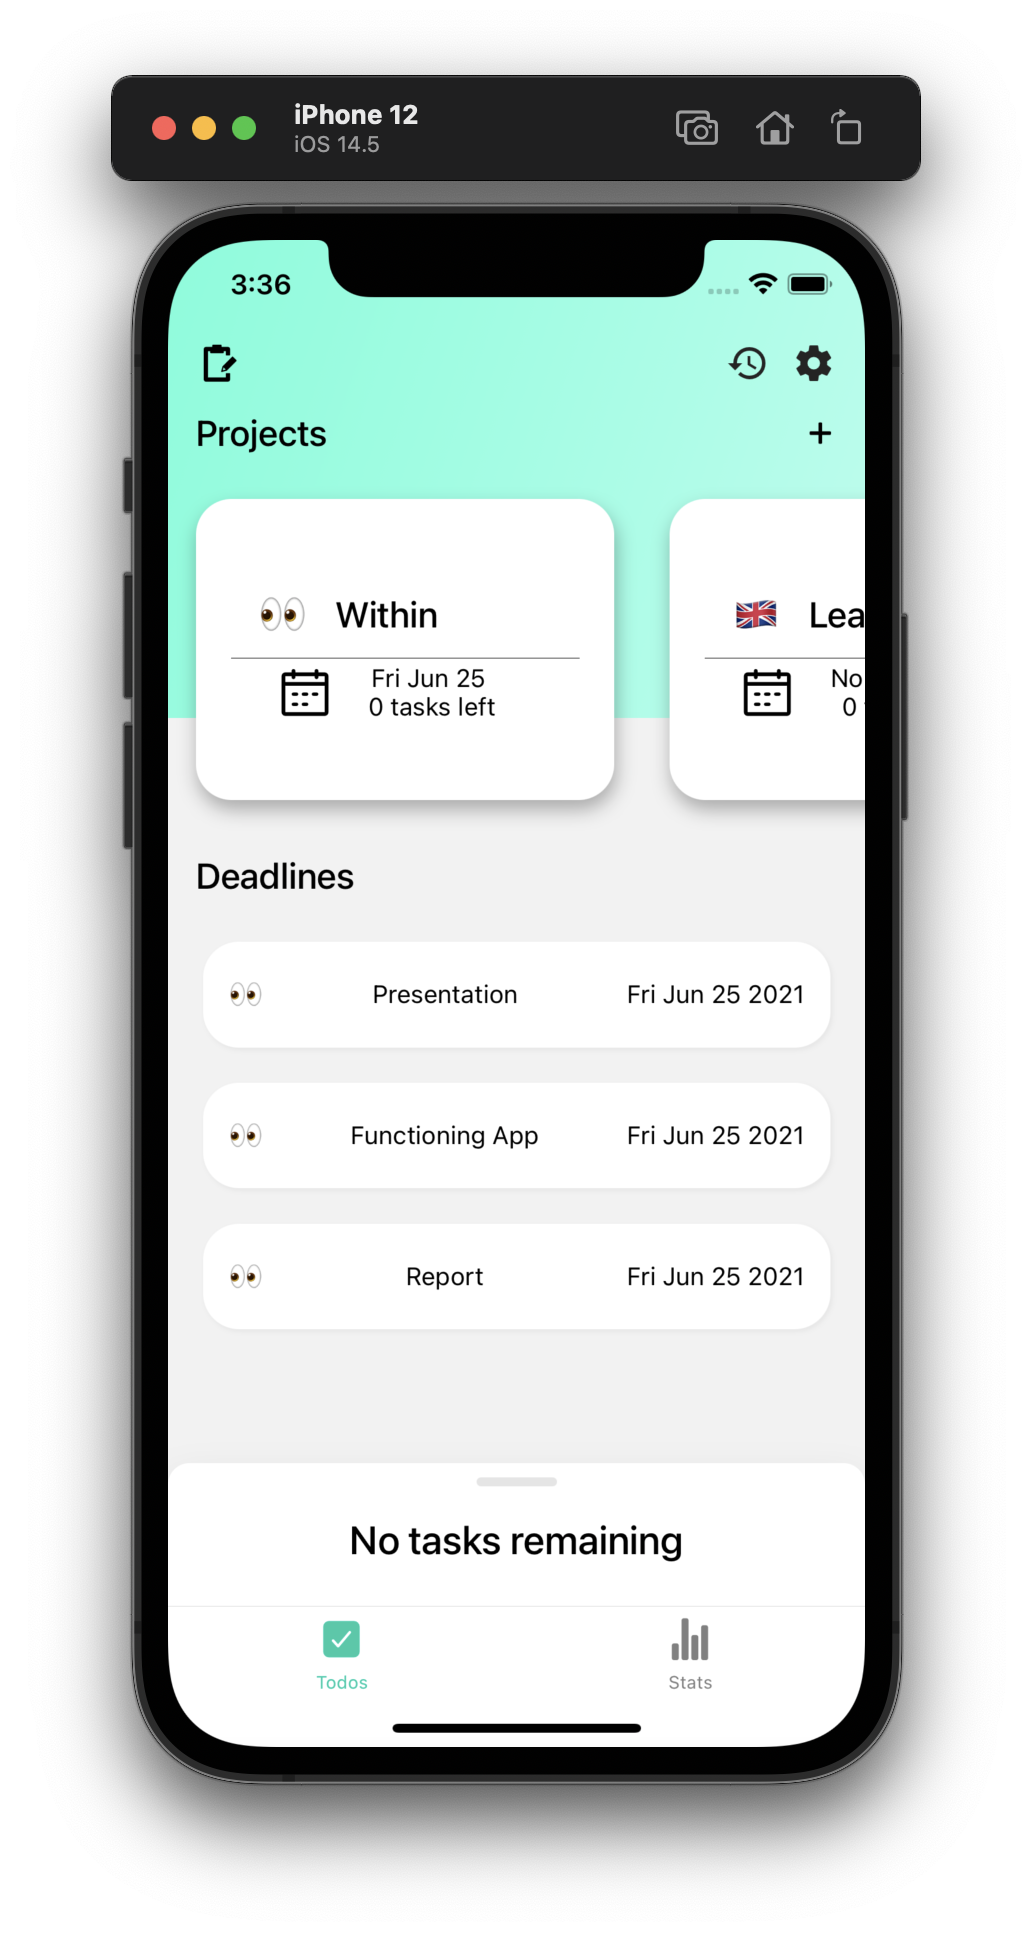
\includegraphics[scale=0.25]{images/home_screen.png}
        \caption{The Within home screen}
        \label{fig:home_screen}
    \end{subfigure}%
\end{figure}

A few noteworthy ways in which the implemented UI conforms to these principles are listed below:

\begin{itemize}
    \item The app focuses itself around a primary color, using slight variations to create contrast to draw user attention. This minimises the gulfs of action, and automates the focus of the user's attention to relevant components.
    \item White space and margins are used to divide screen real-estate into semantically disjoint groups of information, which provides different fields of focus for different user intentions.
    \item Interactive elements will ``hover'' above the screen using drop shadows to convey the concept of elevation\footnote{\href{https://material.io}{Material UI Documentation}}. Elevated components are intuitively ``pressable'', minimising the gulf of execution.
    \item Interactive elements are interfaced with either a short touch, long press or swipe. These conform to many smartphone users' learned behaviours from other popular apps, removing any form of challenge in actuating an intention. Additionally, the most natural and frequent intentions (as determined by user journeys) are actuated with the simplest action (a short press), and require the fewest actions to execute.
    \item All interactive elements provide visual and animated feedback, using a transient opacity or highlight. This provides instant feedback and minimises the gulf of evaluation.
\end{itemize}

The resulting user interface is described by early testers as ``clean and minimal'', providing a much more compact user experience in which users can perform most of the app's base functionality without switching off of the main screen.

\section{Limitations and Issues}
The mechanisms of the Within project have been clearly documented. However, many parts of the application remain untested. Due to the limitations of solo development, testing was only strictly enforced on business logic and database sensitive operations. Ideally, snapshot tests would be implemented to ensure a consistent user interface and experience across different devices. A few known issues are listed below:

\begin{itemize}
    \item Many components in the UI have their dimensions determined as a fraction of the viewport height and width. Some UI components may therefore appear odd on very squarish devices as a result.
    \item Some React components encapsulate a lot of business logic, which may benefit from refactoring.
    \item No easy mechanism is currently in place to easily switch off of Firebase APIs. Refactoring the reducers to fetch data from different sources using a status flag would be much cleaner.
    \item No workaround for the lack of notification blocking functionality on iOS is currently implemented.
    \item Visualisations are not implemented as an active user base has not yet been achieved.
\end{itemize}

Despite these issues, the app now offers a usable base product and is ready for evaluation and iterative development, as we will explore in the next chapter.